\documentclass[11pt]{article}
\usepackage{../EllioStyle}
\usepackage{listings}
\usepackage{mathtools}

\definecolor{codegreen}{rgb}{0,0.6,0}
\definecolor{codegray}{rgb}{0.5,0.5,0.5}
\definecolor{codepurple}{rgb}{0.58,0,0.82}
\definecolor{backcolour}{rgb}{0.95,0.95,0.92}

\graphicspath{ {imgs/} }

\title{Project}
\author{Elliott Pryor}
\date{5 December 2023}

\rhead{Project}
\lhead{Elliott Pryor}

\begin{document}
\maketitle

\problem{1}
Consider the system
$$
G(s) = \frac{50(s+3)}{s(s+2)(s+5)}
$$

\begin{enumerate}[a)]
    \item Use Bode plot to design a lead compensator $C(s)$ with unity DC gain so that the phase margin of the closed-loop system is no less than 40\degree.
    \item Use MATLAB to verify the resulting phase marginally
    \item What is the bandwidth of the resulting closed-loop system?
\end{enumerate}

\begin{figure}[h] 
    \centering
    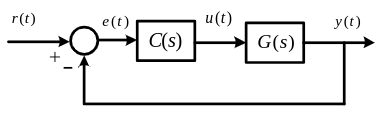
\includegraphics[width=0.55 \linewidth]{12-04-p1.png}
    \caption{Problem1}
    \label{fig:p1}
\end{figure}

\soln

\begin{enumerate}[a)]
    \item Unity DC gain means $K = 1$. 
    \begin{figure}[h] 
        \centering
        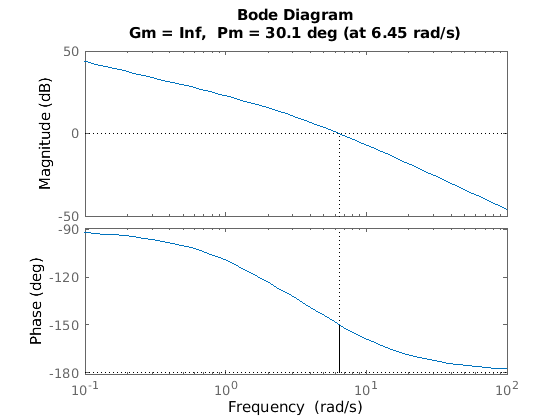
\includegraphics[width=0.55 \linewidth]{p1_bode_1.png}
        \caption{Problem 1: Bode plot of $G(s)$}
        \label{fig:p1_bode_1}
    \end{figure}
    We see that phase margin is 30\degree. 
    So we need to add at least 10\degree of phase margin.
    Choose $\alpha = 1/3$ so $\phi_{max} = 30\degree$ which is less than 60.
    We want $\omega_{max} = \omega_{gc} = 6.45$,
    so then $T = \frac{1}{\omega_{max}\sqrt{\alpha}} = 0.2684$

    So finally $C(s) = \frac{Ts + 1}{\alpha T s + 1} = \frac{0.2684 s + 1}{0.0895s + 1}$
    \item See figure \ref{fig:p1_bode_2} 
    \begin{figure}[h]
        \centering
        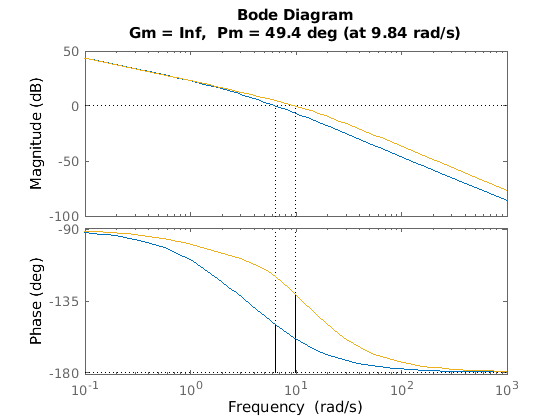
\includegraphics[width=0.55 \linewidth]{p1_bode_2.png}
        \caption{Problem 1: Bode plot of $KC(s)G(s)$ (with lead compensator)}
        \label{fig:p1_bode_2}
    \end{figure}

    \item The bandwidth is the frequency at which the magnitude is $\sqrt{2}/2$ or -3dB.
    We find this at 15.981 rad/s. By looking at the Bode plot of the closed loop system ($\frac{KC(s)G(s)}{1 + KC(s)G(s)}$).
    
\end{enumerate}



\problem{2}
Consider the system
$$
G(s) = \frac{K}{s(s/5 + 1)(s/250 + 1)}
$$
\begin{enumerate}[a)]
    \item Use Bode to design a lag compensator $C(s)$ so that the closed loop system satisfies:
    \begin{itemize}
        \item The steady state error to a unit ramp reference input is less than 0.01
        \item The phase margin is no less than 40\degree
    \end{itemize}
    \item Use MATLAB to verify the resulting phase margin
\end{enumerate}
\begin{figure}[h] 
    \centering
    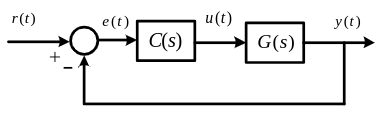
\includegraphics[width=0.55 \linewidth]{12-04-p1.png}
    \caption{Problem2}
    \label{fig:p2}
\end{figure}

\soln

\begin{enumerate}[a)]
    \item So first we need to find gain to make the steady state error within range.
    It is a type 1 system with $L_0 = \frac{1250 K}{(s + 5)(s + 250)}$, so the steady state
    tracking error of unit ramp is $1/L_0(0) = 1/K$, thus $K > 100$.
    We pick $K = 200$.
    
    We plot the Bode of $KG(s)$ and discover a gain margin of 64dB and phase margin of 88.1\degree at $\omega_{gc} = 0.16$ rad/s.
    This already has enough phase margin, so we are done, and we don't need a compensator.

    \item See figure \ref{fig:p2_bode_1} 
    \begin{figure}[h]
        \centering
        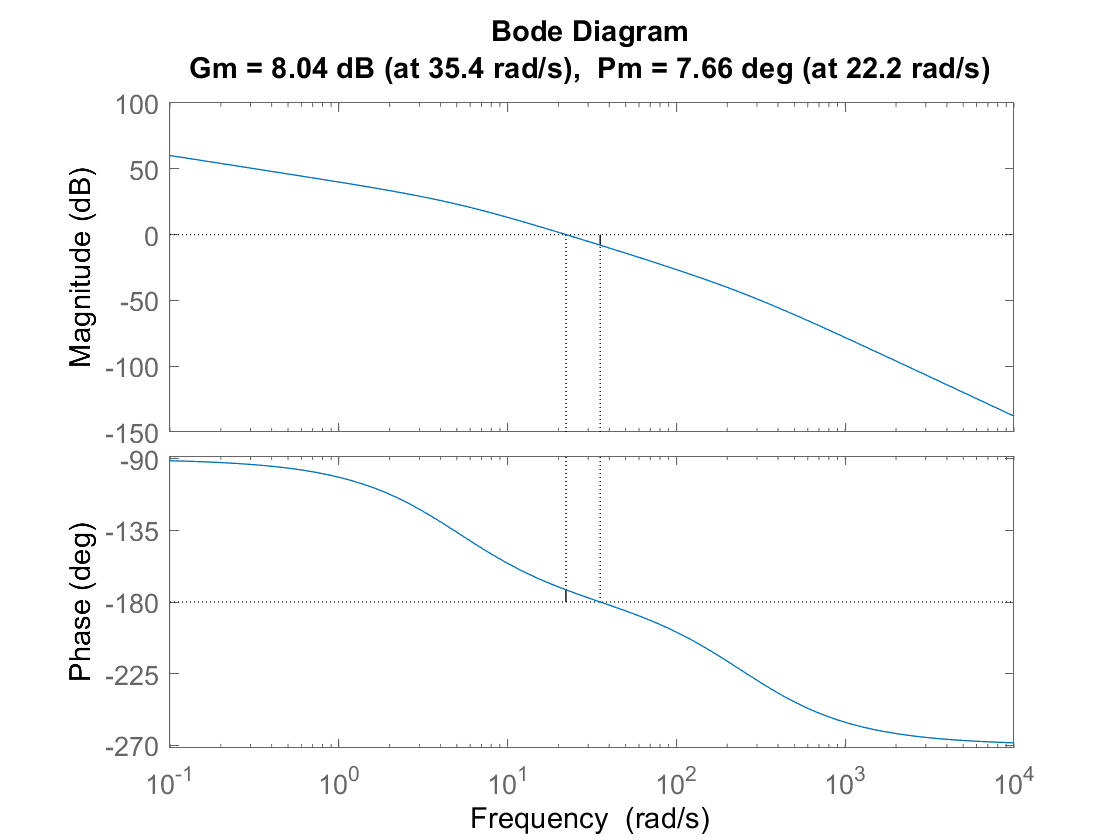
\includegraphics[width=0.55 \linewidth]{p2_bode_1.png}
        \caption{Problem 2: Bode plot of $G(s)$ with $K=200$}
        \label{fig:p2_bode_1}
    \end{figure}
\end{enumerate}









\problem{3}
Given the state space model of a system:

\begin{align*}
    \dot{x} &= \begin{bmatrix}
        2 & 1 \\ -1 & 1
    \end{bmatrix} x + \begin{pmatrix}
        1 \\ 2
    \end{pmatrix} u \\
    y &= \begin{pmatrix}
        1 & 1
    \end{pmatrix} x
\end{align*}

\begin{enumerate}[a)]
    \item Find the state feedback gain $F$ such that the closed-loop system has -1 and -2 at its poles.
    Compute $F$ without using any state transformation.
    \item Design an observer to estimate the state of the system. Select the poles for the error dynamics to be $-2 \pm 2i$
    \item Construct an observer-based output feedback law that stabilizes the system.
\end{enumerate}
\soln

\begin{enumerate}[a)]
    \item We want to design feedback $F$ without using any state transformation.
    So we do this by inspection of the characteristic polynomial.
    We know that the characteristic polynomial is:
    \begin{align*}
        \det(\lambda I - A + BF) &= \begin{vmatrix}
            \lambda - 2 + f_1 & -1 + f_2 \\ 1 + 2f_1 & \lambda - 1 + 2f_2
        \end{vmatrix} \\
        &= (\lambda - 2 + f_1)(\lambda - 1 + 2f_2) - (-1 + f_2)(1 + 2f_1) \\
        &= \lambda^2 - \lambda + 2f_2 \lambda -2 \lambda + 2 - 4 f_2 + f_1 \lambda - f_1 + 2f_1 f_2 + 1 + 2f_1 - f_2 -2f_1f_2 \\
        &= \lambda^2 + (-1 + 2f_2 -2 + f_1)\lambda + (2 - 4f_2 - f_1 + 2f_1f_2 + 1 + 2f_1 - f_2 -2f_1f_2) \\
        &= \lambda^2 + (2f_2 - 3 + f_1)\lambda + (3 -5f_2 + f_1)
    \end{align*}
    So we want the characteristic polynomial to be:
    $(\lambda + 1)(\lambda + 2) = \lambda^2 + 3 \lambda + 2$,
    so $2f_2 + f_1 -3 = 3$ and $f_1 - 5f_2 + 3 = 2$,
    from the first equation we have $f_1 = 6 - 2f_2$, so $6 - 2f_2 - 5f_2 + 3 = 2$,
    which means $f_2 = 1$ and $f_1 = 4$.
    Thus $F = \begin{bmatrix}
        4 & 1
    \end{bmatrix}$

    \item We want to design an observer with poles at $-2 \pm 2i$.
    We can do this in the similar way as above.
    With $\lambda I - A + LC$
    \begin{align*}
        \det(\lambda I - A + LC) &= \begin{vmatrix}
            \lambda - 2 + l_1 & -1 + l_2 \\ 1 + l_1 & \lambda - 1 + l_2
        \end{vmatrix} \\
        &= (\lambda - 2 + l_1)(\lambda - 1 + l_2) - (-1 + l_2)(1 + l_1) \\
        &= \lambda^2 - \lambda + l_2 \lambda -2 \lambda + 2 - 2 l_2 + l_1 \lambda - l_1 + l_1 l_2 +1 + l_2 +l_1 -l_1l_2 \\
        &= \lambda^2 + (-1 + l_2 -2 + l_1)\lambda + (2 - 2l_2 - l_1 + l_1l_2 + 1 + l_2 +l_1 -l_1l_2) \\
        &= \lambda^2 + (l_2 + l_1 - 3)\lambda + (3 - l_2 - 2l_1)
    \end{align*}
    We want the characteristic polynomial to be:
    $\lambda^2 + 4 \lambda + 8$.
    So $l_2 + l_1 -3 = 4$ and $3 - l_2 -2l_1 = 8$.
    From the first we have $l_2 = 7 - l_1$,
    so $3 - 7 + l_1 - 2l_1 = 8 \to l_1 = -12$, and thus $l_2 = 19$
    So $L = \begin{bmatrix}
        -12 \\ 19
    \end{bmatrix}$

    \item We put this all together:
    \begin{align*}
        \begin{bmatrix}
            \dot{x} \\ \dot{\hat{x}}
        \end{bmatrix} &= \begin{bmatrix}
            A - BF & -BF \\ 0 & A - LC
        \end{bmatrix} \begin{bmatrix}
            x \\ \hat{x}
        \end{bmatrix} + \begin{bmatrix}
            B \\ 0
        \end{bmatrix} r \\
        y &= \begin{bmatrix}
            C & 0
        \end{bmatrix} \begin{bmatrix}
            x \\ \hat{x}
        \end{bmatrix}
    \end{align*}
    So we have:
    \begin{align*}
        \begin{bmatrix}
            \dot{x} \\ \dot{\hat{x}}
        \end{bmatrix} &= \begin{bmatrix}
            -2 & 0 & -4 & -1 \\
            -9 & -1 & -8 & -2 \\
            0 & 0 & 14 & 13 \\
            0 & 0 & -20 & -18
        \end{bmatrix} \begin{bmatrix}
            x \\ \hat{x}
        \end{bmatrix} + \begin{bmatrix}
            1 \\ 2 \\ 0 \\ 0
        \end{bmatrix} r \\
        y &= \begin{bmatrix}
            1 & 1 & 0 & 0
        \end{bmatrix} \begin{bmatrix}
            x \\ \hat{x}
        \end{bmatrix}
    \end{align*}
\end{enumerate}






\problem{4}
Complete the class evaluation:
\soln

Yes

\newpage
\large{\textbf{Code Appendix}}
\lstdefinestyle{mystyle}{
%    backgroundcolor=\color{backcolour},   
    commentstyle=\color{codegreen},
    keywordstyle=\color{magenta},
    numberstyle=\tiny\color{codegray},
    stringstyle=\color{codepurple},
    basicstyle=\ttfamily\footnotesize,
    breakatwhitespace=false,         
    breaklines=true,                 
    captionpos=b,                    
    keepspaces=true,                 
    numbers=left,                    
    numbersep=5pt,                  
    showspaces=false,                
    showstringspaces=false,
    showtabs=false,                  
    tabsize=2
}
\lstset{style=mystyle}
\lstinputlisting[language=Octave]{code.m}

\end{document}